\documentclass{article}
\usepackage{graphicx}
\usepackage{float}

\title{COMP1044 Coursework Assignment 2 Report A \\ Group 15 / Chew Language}
\author{
	Leong Chang Yung, 20307078
	\and
	Lucas Dylan Purnell, XXXXXXXX
	\and
	Tan Zhun Xian, 20313854
	\and
	Hao Wei, XXXXXXXX
	\and
	Morhaf, XXXXXXXX
	\and
	Thomas Tan Kean Yew, 20316601
}
\date{\today}

\begin{document}
\maketitle
\newpage
\section{Database Design Diagram}
	\begin{figure}[H]
		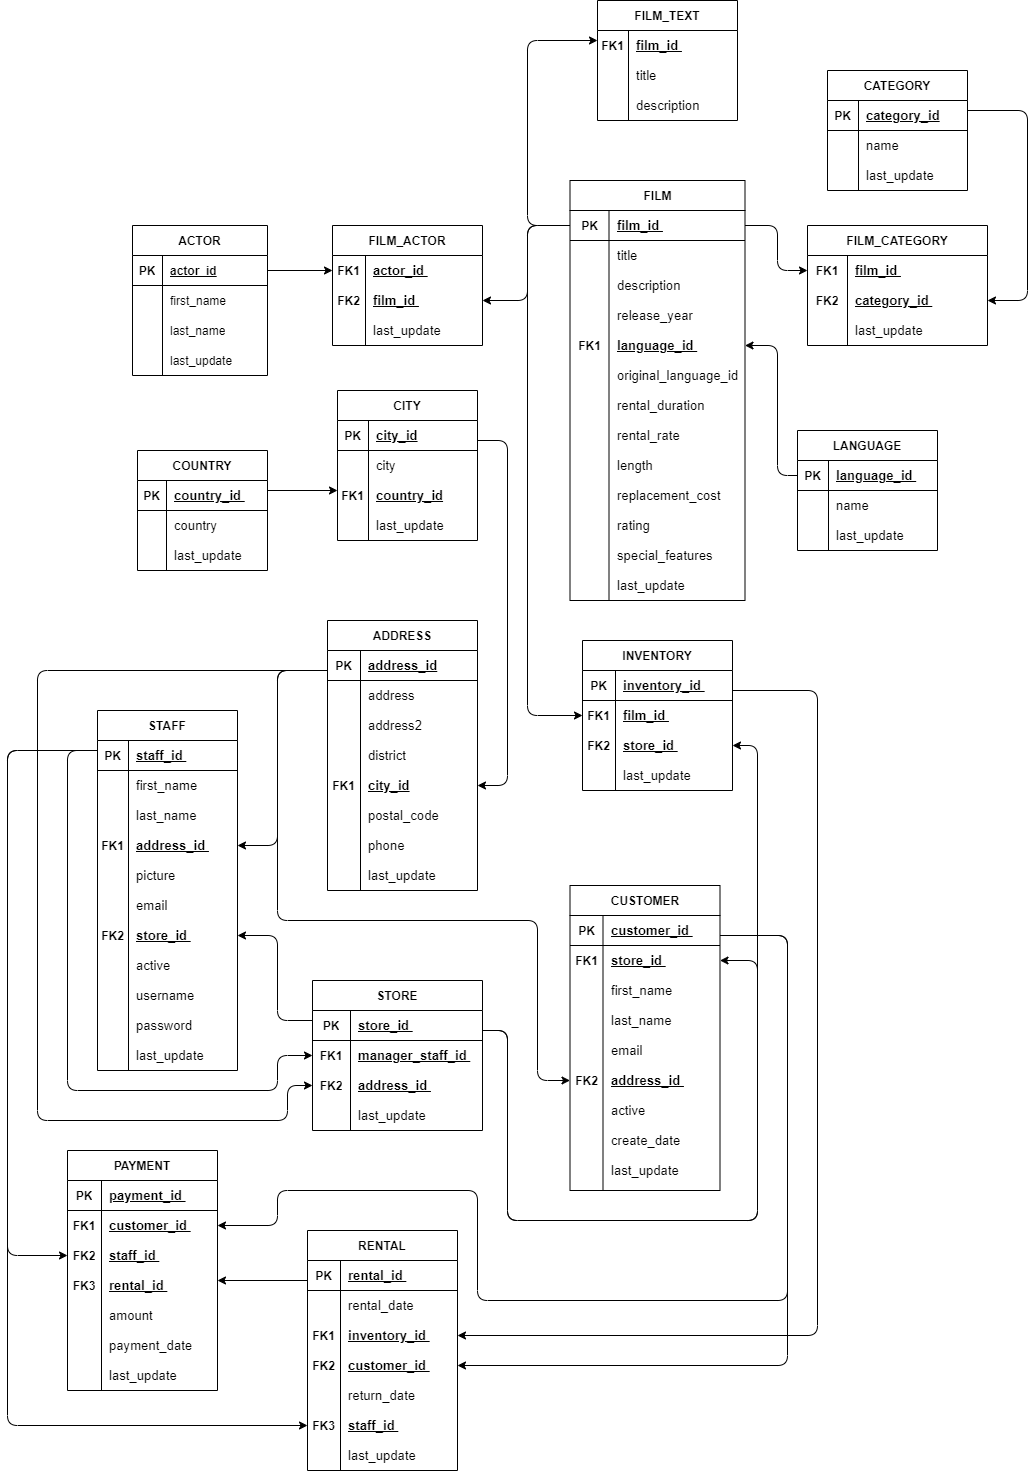
\includegraphics[width=\textwidth]{DBI CourseworkA}
		\caption{Proposed model for database.}	
	\end{figure}
		
\section{Datatype Selection}
	For every field we chose the datatype depending on what would both match the data we had available and take up the lowest amount of memory possible 
	while still ensuring that the type and length would be suitable for all new entries. 
	\\\\
	For most of the fields that were purely filled with numbers we set the type to either \textbf{int} or \textbf{decimal} (depending on whether the number was an integer 
	or a decimal). A few examples of this are the \emph{id} fields and the \emph{length} and \emph{rating} field in the \emph{film} table. A notable exception to this was the 
	\emph{phone number} field. We set this datatype to \textbf{varchar} to allow people to enter their phone numbers in a different format despite all phone numbers in the 
	dataset being integers. This was because many phone numbers need either a plus or a dash. Additionally, this field could be parsed and converted into an integer later if needed.
	\\\\	
	For all \textbf{varchar} we used the same principle but for the majority of fields we tried to keep the maximum lengths in neat values (normally multiples of 5). For instance, common 
	values for the maximum length of \textbf{varchar} are 10, 25 and 50. We decided to set each field’s maximum length to the longest realistic input value.
	For instance, we set \emph{film\textunderscore title} to \textbf{varchar(100)} as the longest name for a popular movie was 76 characters. We also set \emph{first\textunderscore name} and 
	\emph{last\textunderscore name} to 50 as we thought that would be a good estimate based on actual estimates of the longest person names.
	\\\\
	All date values were set to the type \textbf{datetime} according to their date and time content. For instance the \emph{last\textunderscore update} and
	\emph{create\textunderscore date} fields.
	
\section{Reasoning for Primary and Foreign Key Choice}
	When we were deciding on what to pick for the primary key for each time we understood that it had to be both unique and non-null. 
	This is because the primary key serves as the identifier for each record in the table and if it is either repeated or \textsc{null} it can no longer serve as an identifier. 
	The obvious candidate here was  the ID field in every table (for instance the \emph{inventory\textunderscore id} in the inventory table) as it fulfils both of these criteria.
	\\\\
	The foreign key has the same requirements except that it need not be unique – only the primary key it references has to be unique. 
	With the in mind we can use the same fields that we used as primary keys. Therefore for each of our arrays the \emph{id} column is used to link the tables together. 
	For instance, \emph{customer\textunderscore id} was chosen as the foreign key to link the \emph{payment} table with the \emph{customer} table and \emph{address\textunderscore id} 
	was chosen as the foreign key to link the \emph{staff} table with the \emph{address} table.

\section{Completeness of the Dataset}
	The database was relatively complete and we did not struggle with the quality of the data. We found that the data values were consistent across the different tables. This meant
	 that we didn’t run into any issues regarding the foriegn keys and we didn’t find conflicting information in the data set.
	\\\\
	We found a few different ways that the dataset was incomplete. The first was missing numbers from the auto-incremental data. For instance,
	 there were missing \emph{address\textunderscore id}’s in \emph{Address.csv}. This problem was easily remedied by enabling the property to \textbf{auto increment} during the creation of said file. 
	\\\\
	The next problem was
	 that many \textsc{null} fields were invalid and are supposed to contain a value. 
	For instance, some of the fields of \emph{Rental\textunderscore id} in \emph{Payment.csv} were \textsc{null} when this should not have been the case. This is a problem as it 
	may compromise the integrity
	 of the database, as these \textsc{null} fields will lead to orphaned records due to the lack of a foriegn key.
	\\\\
	There was also a \textsc{null} value in the \emph{password} column of the \emph{staff.csv} table. This would indicate data corruption, data loss, or staff negligence in inputting a proper password. In the interest of system security, the best remedy would be to get the relevant staff member to provide a value for this \textsc{null} field. However, while the problem stands, we decided that it would be better to leave these fields as \textsc{null} to avoid risking data integrity.

\section{Errors in the Database}
	We also noticed that in \emph{country.csv} and \emph{customer.csv} that there wasn’t a consistent delimiter. The file alternated between using commas 
	and semicolons to separate data. The lack of support for semicolon delimiters made it impossible to import the data into the database while keeping it in its intended format. 
	To remedy this we replaced the semicolons with commas wherever applicable using text editors.
	\\\\
	The other error was the existence of a corrupted picture file within \emph{staff.csv}. This corruption made it impossible to view or display the aforementioned picture. 
	We decided that leaving a corrupted picture within the staff database was not of high importance and wouldn’t decrease the completeness or understandability of the dataset,
	so we just removed the picture. A partial solution was found in making the field type storing the picture as \textbf{longblob}. 
	\begin{figure}[H]
		
\includegraphics[width=13cm]{staff-picture}
		\caption{The partially recovered staff photo.}
	\end{figure}
	This allowed the picture to be imported, albeit still in an incomplete state. 

\section{Conclusion}
	At the point of writing, the team determined the database to be sufficient for further usage, due to SELECT queries functioning properly when used to select specific rows in the tables.


\end{document}